\chapter{The Gaussian Toolkit Pipeline}
\label{ch:pipeline}

This chapter describes the architecture, implementation, and operational characteristics of the \texttt{gaussian-toolkit}, the end-to-end reconstruction pipeline developed for this project. The toolkit integrates the technologies described in Chapter~\ref{ch:technology} into a cohesive, containerised workflow with a web-based user interface and AI-assisted orchestration.

\section{Pipeline Architecture}
\label{sec:pipe-arch}

The \texttt{gaussian-toolkit} implements a six-stage pipeline, shown schematically in Figure~\ref{fig:pipeline-overview}:

\begin{enumerate}
  \item \textbf{Video ingestion and frame extraction.} Source video is decoded and frames are extracted at a configurable rate using FFmpeg. Blurred and redundant frames are optionally filtered using a Laplacian variance threshold.

  \item \textbf{Structure-from-Motion.} Extracted frames are processed by \acrshort{colmap} to produce camera poses and a sparse point cloud (Section~\ref{sec:tech-sfm}).

  \item \textbf{Gaussian Splat training.} The sparse point cloud and camera poses initialise a \acrshort{3dgs} training run, producing the Gaussian splat representation (Section~\ref{sec:tech-3dgs}).

  \item \textbf{Mesh extraction} (optional). The trained Gaussian representation is processed through one or more mesh extraction methods to produce explicit surface geometry (Section~\ref{sec:tech-mesh}).

  \item \textbf{Post-processing and export.} Results are exported in standard formats: \texttt{.ply} and \texttt{.splat} for Gaussian representations, \texttt{.glb}/\texttt{.gltf} and \texttt{.usd} for meshes.

  \item \textbf{Viewing and delivery.} An integrated web viewer provides immediate browser-based viewing of splat results; mesh results can be loaded in Blender, Unreal Engine, or any compatible 3D application.
\end{enumerate}

\begin{figure}[htbp]
  \centering
  % Placeholder for pipeline diagram
  \begin{tikzpicture}[
    node distance=1.5cm,
    block/.style={
      rectangle, rounded corners=3pt,
      draw=MidGrey, fill=LightGrey,
      text width=3.2cm, minimum height=1.2cm,
      align=center, font=\small\sffamily
    },
    arrow/.style={-{Stealth[length=3mm]}, thick, MidGrey}
  ]
    \node[block, fill=UoSRed!10, draw=UoSRed] (ingest) {Video\\Ingestion};
    \node[block, right=of ingest] (sfm) {COLMAP\\SfM};
    \node[block, right=of sfm] (train) {3DGS\\Training};
    \node[block, right=of train, fill=DreamLabAccent!10, draw=DreamLabAccent] (view) {Browser\\Viewer};
    \node[block, below=0.8cm of train] (mesh) {Mesh\\Extraction};
    \node[block, right=of mesh, fill=DreamLabAccent!10, draw=DreamLabAccent] (export) {Blender/\\Unreal};

    \draw[arrow] (ingest) -- (sfm);
    \draw[arrow] (sfm) -- (train);
    \draw[arrow] (train) -- (view);
    \draw[arrow] (train) -- (mesh);
    \draw[arrow] (mesh) -- (export);

    \node[above=0.3cm of ingest, font=\tiny\sffamily\color{MidGrey}] {Stage 1};
    \node[above=0.3cm of sfm, font=\tiny\sffamily\color{MidGrey}] {Stage 2};
    \node[above=0.3cm of train, font=\tiny\sffamily\color{MidGrey}] {Stage 3};
    \node[above=0.3cm of view, font=\tiny\sffamily\color{MidGrey}] {Stage 4a};
    \node[below=0.3cm of mesh, font=\tiny\sffamily\color{MidGrey}] {Stage 4b};
    \node[below=0.3cm of export, font=\tiny\sffamily\color{MidGrey}] {Stage 5};
  \end{tikzpicture}
  \caption{Schematic overview of the \texttt{gaussian-toolkit} pipeline. The primary pathway (top) produces browser-viewable splat representations; the secondary pathway (bottom) produces exportable meshes for traditional 3D workflows.}
  \label{fig:pipeline-overview}
\end{figure}

\section{Docker Containerisation}
\label{sec:pipe-docker}

The pipeline is containerised using Docker Compose, with the system decomposed into multiple services to manage conflicting dependency requirements:

\begin{description}
  \item[Main container (\texttt{gaussian-toolkit})] Hosts \acrshort{colmap}, the primary \acrshort{3dgs} training implementations (original, \acrshort{mrnf}, \acrshort{mcmc}), \acrshort{tsdf} mesh extraction, the web interface, and the 3D viewer. Based on NVIDIA's CUDA 12.1 development image with Ubuntu 22.04.

  \item[MILo sidecar (\texttt{milo-service})] A separate container running the MILo mesh extraction service, which requires a distinct Python environment (PyTorch 2.1 with specific CUDA toolkit versions) incompatible with the main container's dependencies. Communication between the main container and MILo sidecar occurs via a shared Docker volume and a lightweight REST API.

  \item[Viewer service (\texttt{splat-viewer})] An Nginx-based container serving the static browser-based splat viewer, with WebSocket support for live progress updates during training.
\end{description}

\begin{technote}
The total Docker image size is approximately 18\,GB for the main container and 12\,GB for the MILo sidecar. While substantial, this is a one-time download cost that eliminates the hours-long dependency installation and debugging process that characterises manual setup of GPU-accelerated 3D reconstruction environments. On a system with NVIDIA Container Toolkit pre-installed, the entire pipeline can be operational within 30 minutes of cloning the repository.
\end{technote}

\section{Agentic Orchestration}
\label{sec:pipe-agent}

A distinguishing feature of the \texttt{gaussian-toolkit} is its use of agentic AI orchestration via Claude Code (Anthropic). Rather than requiring users to manually configure pipeline parameters, manage intermediate outputs, and diagnose failures, the pipeline exposes a set of structured tool interfaces that an AI agent can invoke to:

\begin{itemize}
  \item Analyse source video characteristics (resolution, frame rate, motion profile) and recommend frame extraction parameters.
  \item Configure \acrshort{colmap} matching strategy based on the image collection structure (sequential for video, exhaustive for unordered photo sets).
  \item Select and parameterise the \acrshort{3dgs} training variant based on the reconstruction requirements.
  \item Monitor training progress and detect convergence or failure conditions.
  \item Invoke mesh extraction with appropriate parameters.
  \item Generate summary reports with quality metrics and visual comparisons.
\end{itemize}

This agentic layer does not replace expert knowledge but encodes common decision patterns into an automated workflow, significantly reducing the time-to-result for routine reconstructions and providing guided assistance for non-specialist operators.

\begin{lstlisting}[language=bash, caption={Example agentic invocation of the pipeline.}, label={lst:agent-invoke}]
# The agent analyses the source and configures the full pipeline
gaussian-toolkit process \
  --input gallery_walkthrough.mp4 \
  --output ./results/ \
  --agent-mode auto \
  --training-method mrnf \
  --mesh-extraction milo \
  --viewer-port 8080
\end{lstlisting}

\section{Web Interface and 3D Viewer}
\label{sec:pipe-viewer}

The \texttt{gaussian-toolkit} includes a web-based interface that provides:

\begin{itemize}
  \item \textbf{Upload and management.} Users can upload source videos, monitor processing progress, and manage multiple reconstruction projects.
  \item \textbf{Real-time training visualisation.} During \acrshort{3dgs} training, periodic renders from novel viewpoints are streamed to the browser, allowing users to assess reconstruction quality as training progresses.
  \item \textbf{Interactive 3D viewing.} Completed splat reconstructions are viewable directly in the browser via an integrated WebGL viewer supporting orbit, pan, and zoom navigation.
  \item \textbf{Comparison mode.} Multiple reconstruction results (e.g., different training methods or parameter settings) can be displayed side-by-side for quality comparison.
  \item \textbf{Export.} Results can be downloaded in standard formats for use in external applications.
\end{itemize}

The viewer is built on a custom WebGL renderer optimised for Gaussian splat rendering, supporting scenes of up to 5 million Gaussians at interactive frame rates on mid-range hardware (NVIDIA RTX 3060 or equivalent). For larger scenes, a progressive level-of-detail system loads Gaussians incrementally based on their contribution to the current view.

\begin{figure}[htbp]
  \centering
  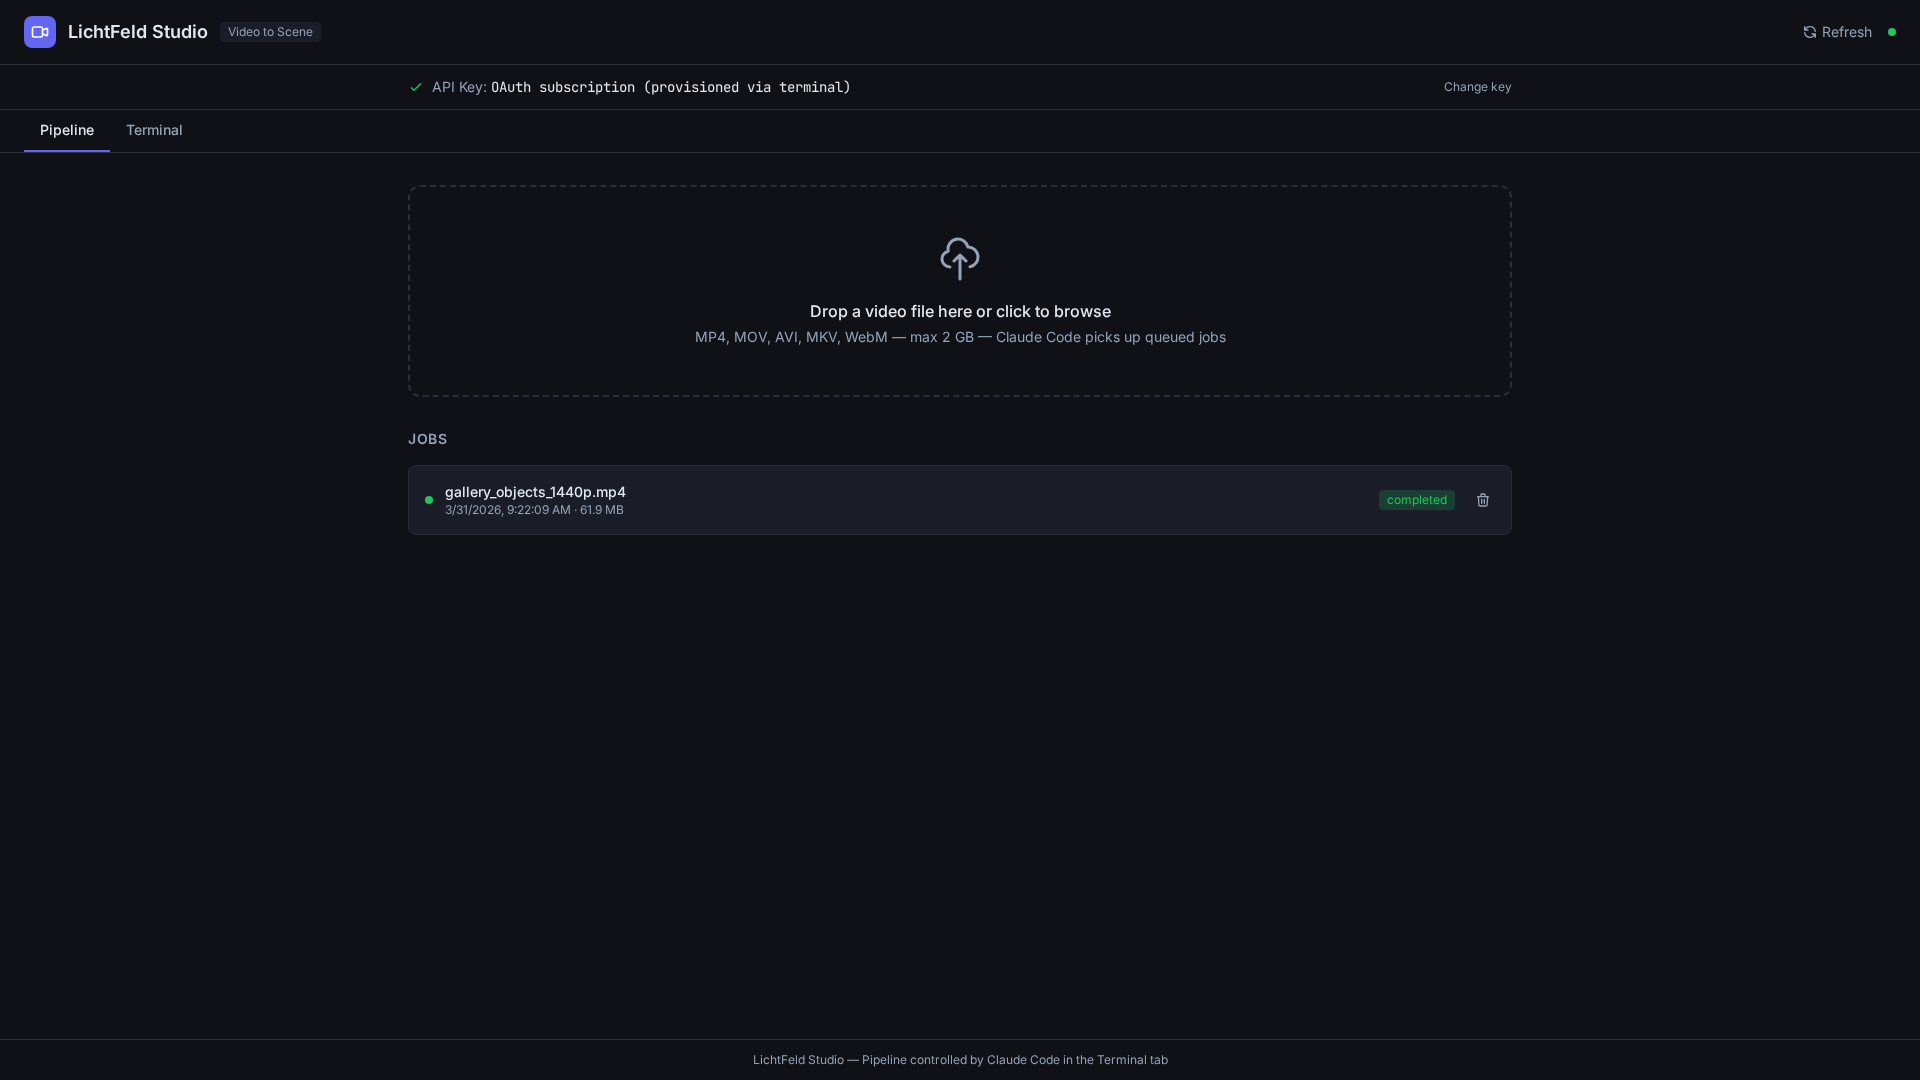
\includegraphics[width=0.48\textwidth]{figures/web_ui_main.png}
  \hfill
  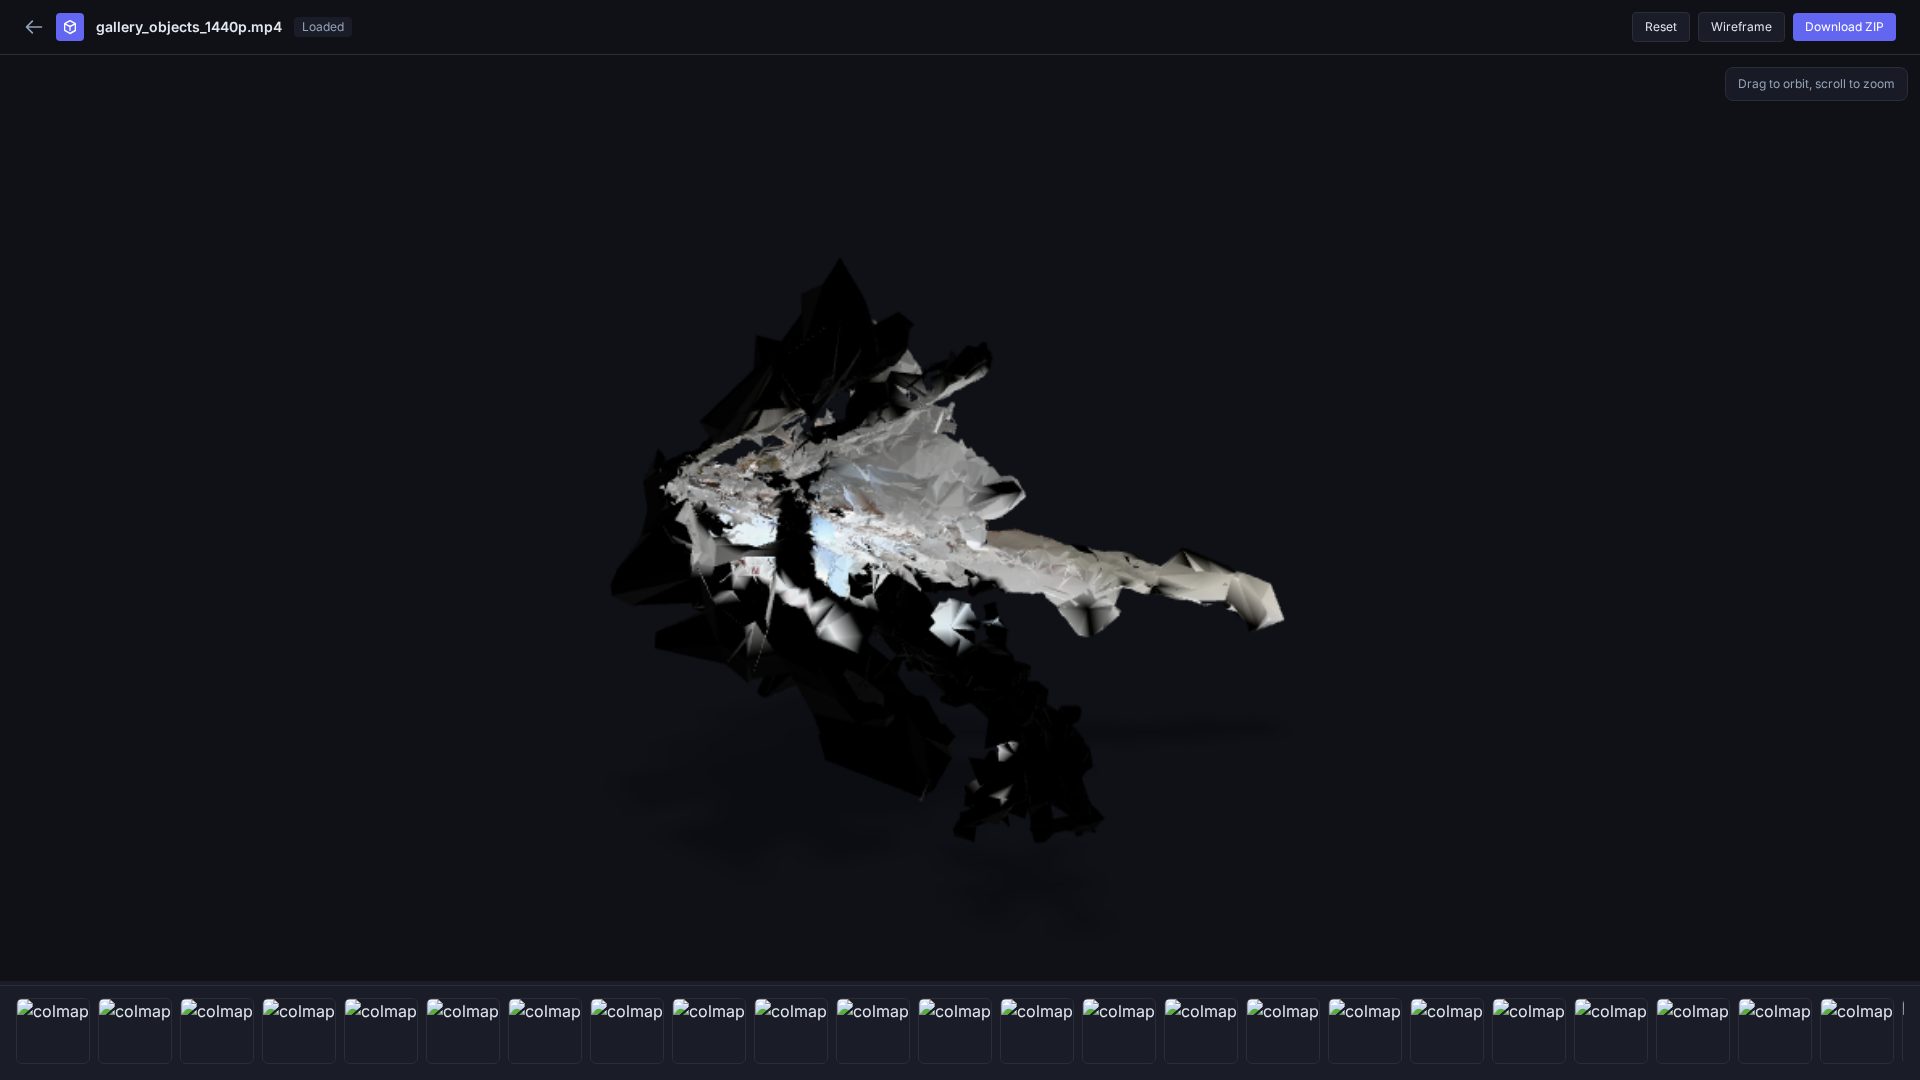
\includegraphics[width=0.48\textwidth]{figures/web_ui_viewer.png}
  \caption{The \texttt{gaussian-toolkit} web viewer displaying an interactive Gaussian splat reconstruction. Users can orbit, pan, and zoom freely within the reconstructed scene.}
  \label{fig:viewer-screenshot}
\end{figure}
